\chapter{Method}
\label{chap:Method}

\begin{itemize}
    \item Explanation of larsoft/Pandora - don't really know..
    \item Explain ESTAR method \cite{ESTAR_Database}
    \item Compare/reference previous methods too? 
\end{itemize}

\section{Overview}

\textcolor{red}{ADDITIONAL DETAIL ON EARLIER STEPS??}

To estimate the reconstructed shower energy, the hits from the shower are found and integrated over to obtain the collected charge in \Gls{adc} units. This is then converted to a conventional charge (number of electrons) by a calibration factor. The reconstruction is done on a per-hit basis which means that any corrections are done for each individual hit and the reconstructed energy of each hit is calculated. The total shower energy is then found by summing up the energy of all associated hits. 

Detector effects such as electron lifetime and recombination must also be considered. The drifting electrons have a finite lifetime in the detector because they will eventually attach to positively charged impurities in the argon \cite{ArgoNeuT_electron_lifetime_paper}. Due to this, the collected charge has to be corrected to account for the electron lifetime. The other effect to consider is electron recombination. When argon atoms are ionised, the resulting argon ion and ionised electron may immediately recombine. This is known as the recombination effect and the magnitude of the effect is largely due to the local electric field \cite{ArgoNeuT_recombination_paper}. The recombination effect is modelled by the Modified Box recombination model and is given by
\begin{equation}\label{eqn:ModBox}
    \frac{dE}{dx} = \frac{\exp{(\frac{\beta}{\rho \mathcal{E}} W_{ion}.\frac{dQ}{dx}}) - \alpha}{\frac{\beta}{\rho \mathcal{E}}},
\end{equation}
where $\frac{dE}{dx}$ is the deposited energy per unit length, $\frac{dQ}{dx}$ is the deposited charge per unit length,  $\mathcal{E}$ is the electric field in the detector, $\rho$ is the density of liquid argon, $W_{ion} = 23.6$ eV which is the energy required to ionise an argon atom, $\alpha = 0.93 \pm 0.02$ and $\beta = 0.212 \pm 0.002$ (kV/cm)(g/cm$^2$)/MeV. The values for parameters $\alpha$ and $\beta$ are results from the \Gls{argoneut} experiment \cite{ArgoNeuT_recombination_paper}.

To convert the collected charge to energy, we will use the Modified Box recombination model in conjunction with the ESTAR database. The ESTAR database is provided by the \Gls{nist} and gives the track length of electrons in liquid argon for energies ranging from 0.01 MeV to 1000 MeV \cite{ESTAR_Database}. This allows $\frac{dE}{dx}$ values to be calculated by dividing the energy by the track length for each entry in the ESTAR database. The deposited charge, Q, is then found by using \EquationRef{eqn:ModBox} to find $\frac{dQ}{dx}$ and multiplying by the track length, \textit{dx}. This now allows the deposited charge and energy to be related. If $\mathcal{E}$ in \EquationRef{eqn:ModBox} is taken to be a variable, the above process is repeated whilst iterating over set values of $\mathcal{E}$. This results in a 3D curve relating both the deposited charge and electric field to energy as is shown in \FigureRef{fig:ESTAR lookup curve}. The energy is interpolated from the deposited charge and electric field. A direct recombination correction is not required with this method as it has already been accounted for in the lookup curve. 

\begin{figure}[h]
    \centering
    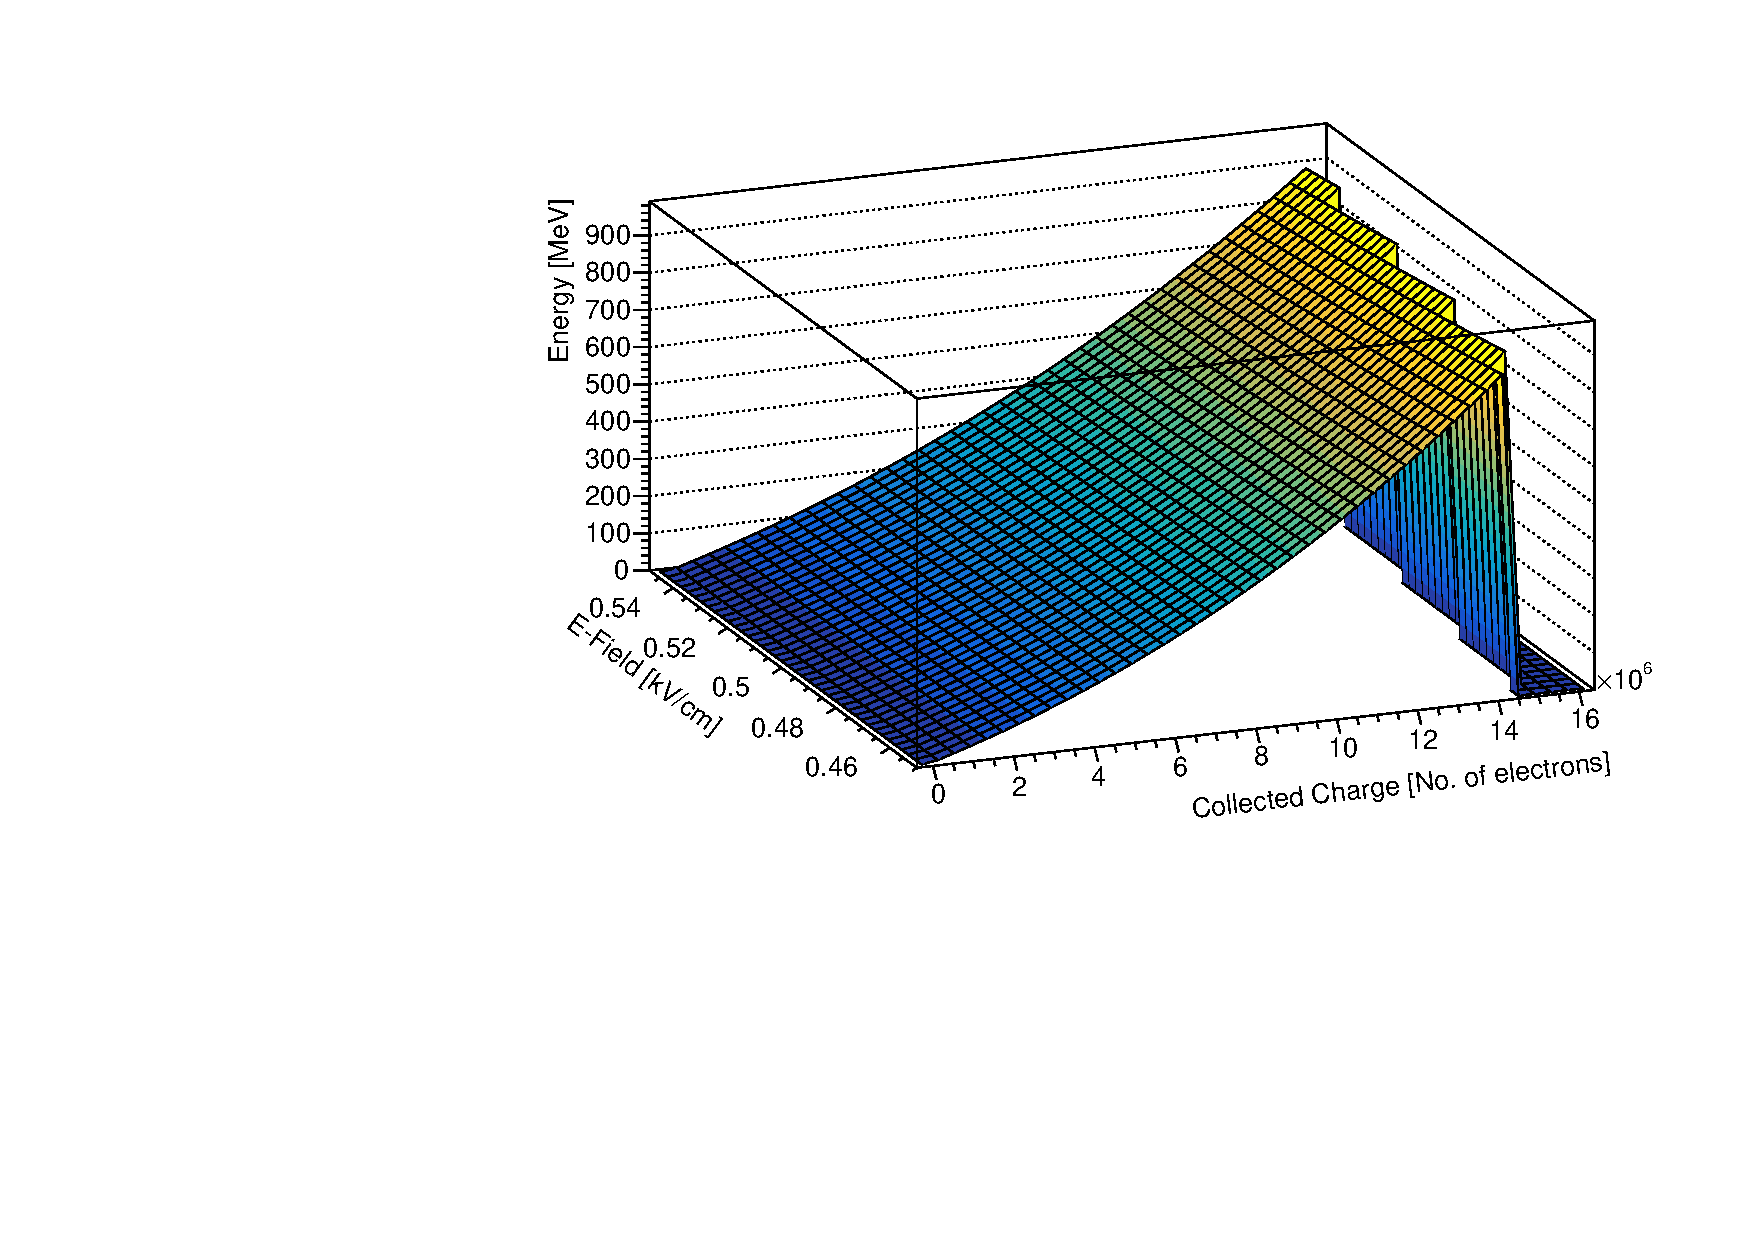
\includegraphics[width = \largefigwidth]{Figures/ESTAR_lookup_curve.pdf}
    \caption{The collected energy as a function of the collected charge and the local electric field. Produced with data from the ESTAR database and use of the Modified Box recombination model.}
    \label{fig:ESTAR lookup curve}
\end{figure}

\newpage
\section{Correcting for SCE}
Since the \gls{sce} causes the electric field in the detector to be non-uniform, the local electric field at each point in the detector needs to be known. An example map of the electric field in the centre of \gls{sbnd} is shown in \FigureRef{fig:SCE map}. To account for each hit being associated with a different value of the electric field, the corresponding \Glspl{sp} for each of the hits are found and the coordinates of the \glspl{sp} in the detector are determined. Instead of using the nominal value for $\mathcal{E}$, the local value for $\mathcal{E}$ at the position of the \Glspl{sp} is used when interpolating the energy. In the case that a hit has no corresponding \Glspl{sp}, the charge weighted centre of the shower is found and the local value of $\mathcal{E}$ at this point is used instead. The charge weighted centre is defined as $\frac{\sum (charge \times position)}{\sum charge}$ from the available \glspl{sp}.

\begin{figure}[h]
    \centering
    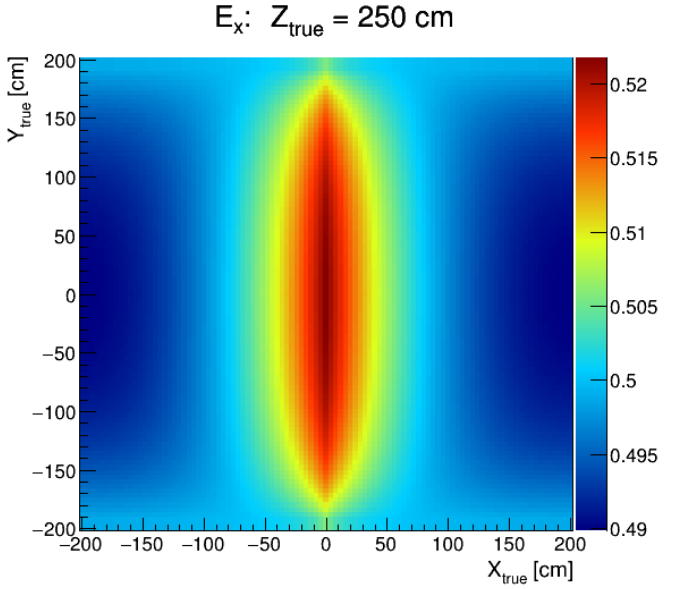
\includegraphics[width = \largefigwidth]{Figures/SCE_map_SBND.png}
    \caption{The expected electric field offset relative to the nominal value of 0.5 kV/cm at z = 250cm in SBND (the centre of the detector) caused by SCE.}
    \label{fig:SCE map}
\end{figure}

















